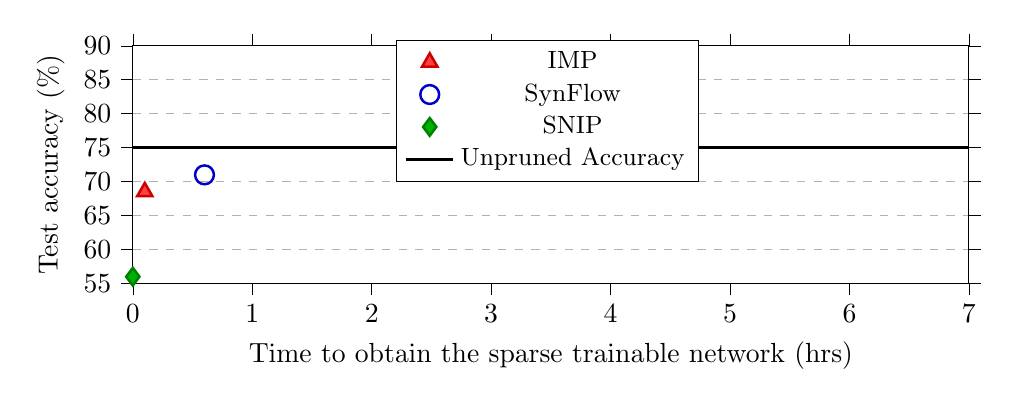
\begin{tikzpicture}
\begin{axis}[
    width=12.2cm,
    height=4.6cm,
    xmin=0, xmax=7,
    ymin=55, ymax=90,
    xtick={0,1,2,3,4,5,6,7},
    ytick={55,60,65,70,75,80,85,90},
    axis lines=box,
    ymajorgrids,
    grid style={gray!60,dashed},
    xlabel={Time to obtain the sparse trainable network (hrs)},
    ylabel={Test accuracy (\%)},
    tick align=outside,
    tick style={black},
    legend style={
        draw=black, fill=white, rounded corners=0pt,
        at={(axis cs:2.2,70)}, anchor=south west,
        font=\small
    },
    every axis plot/.append style={line width=0.9pt},
]

% IMP (triangle, red)
\addplot[
    only marks,
    mark=triangle*,
    mark size=3.2pt,
    draw=red!80!black, fill=red!75
] coordinates {(0.10,68.5)};
\addlegendentry{IMP}

% SynFlow (circle, blue)
\addplot[
    only marks,
    mark=o,
    mark size=3.4pt,
    draw=blue!80!black, fill=white
] coordinates {(0.60,71.0)};
\addlegendentry{SynFlow}

% SNIP (diamond, green)
\addplot[
    only marks,
    mark=diamond*,
    mark size=3.2pt,
    draw=green!50!black, fill=green!70!black
] coordinates {(0.00,56.0)};
\addlegendentry{SNIP}

% Unpruned accuracy (black horizontal line)
\addplot[black, very thick] coordinates {(0,75) (7,75)};
\addlegendentry{Unpruned Accuracy}

\end{axis}
\end{tikzpicture}